\chapter{Other Element Quality Metrics\label{s:other-el}}

In addition to triangular, quadrilateral, tetrahedral, and hexahedral
elements, \verd\ also provides volume computation for other element
types, namely: pyramids (with quadrilateral base), wedges, and knives,
respectively illustrated
in Figures~\ref{f:pyr}, \ref{f:wed}, and~\ref{f:kni}. Note that
\texttt{vtkMeshQuality} does not support these element types. 

\begin{figure}[htb]
  \centering
  \includegraphics[width=2in]{pyramid}
  \caption{Numbering of vertices and edges on a pyramidal element.%
                                                                  \label{f:pyr}}
\end{figure}

\begin{figure}[htb]
  \centering
  \includegraphics[width=2in]{wedge}
  \caption{Numbering of vertices and edges on a wedge element.%
                                                                  \label{f:wed}}
\end{figure}

\begin{figure}[htb]
  \centering
  \includegraphics[width=2in]{knife}
  \caption{Numbering of vertices and edges on a knife element.%
                                                                  \label{f:kni}}
\end{figure}

The volume $V$ of any of these elements is calculated by decomposing them in
a tetrahedral partition, as follows:
\begin{itemize}
\item
pyramids are divided into 2 tetrahedra,
\item
wedges are divided into 3 tetrahedra, and
\item
knives are divided into 4 tetrahedra.
\end{itemize}

Further, we define a \emph{unit pyramid} as a pyramid whose triangular faces
are equilateral triangles with unit edge length. Note that this
entails that the quadrilateral face is a unit square, thus making the
unit pyramid a special case of regular pyramid.

Finally, we define a \emph{unit wedge} as a wedge whose quadrilateral
faces are unit squares. Note that this entails that the 2 triangular
faces are equilateral triangles with unit edge length, thus making the
unit wedge a special case of right triangular prism.
% -------------------Metric Table-------------------
\newcommand{\othermetrictable}[8]{%
  \begin{center} 
  \begin{tabular}{ll}
    \multicolumn{2}{r}{\textbf{\sffamily\Large #1}}\\\hline
    Dimension:                           & #2\\ 
    Acceptable Range:                    & #3\\ 
    Normal Range:                        & #4\\ 
    Full Range:                          & #5\\ 
    $q$ for unit element:                & #6\\
    Reference:                           & #7\\
    \verd\ function:       & \texttt{#8}\\ \hline
  \end{tabular} 
  \end{center}
}

\clearpage
\newpage %---------------------------Volume-----------------------------
\section{Pyramid Volume}

The pyramid volume metric is simply
\[
q = V.
\]

\othermetrictable{volume}%
{$L^3$}%                                      Dimension
{$[0,DBL\_MAX]$}%                             Acceptable range
{$[-DBL\_MAX,DBL\_MAX]$}%                     Normal range
{$[-DBL\_MAX,DBL\_MAX]$}%                     Full range
{$\frac{1}{3\sqrt{2}}$}%                      Unit element
{--}%                                         Citation
{v\_pyramid\_volume}%                         Verdict function name

\newpage %---------------------------Volume-----------------------------
\section{Wedge Volume}

The wedge volume metric is simply
\[
q = V.
\]

\othermetrictable{volume}%
{$L^3$}%                                      Dimension
{$[0,DBL\_MAX]$}%                             Acceptable range
{$[-DBL\_MAX,DBL\_MAX]$}%                     Normal range
{$[-DBL\_MAX,DBL\_MAX]$}%                     Full range
{$\frac{\sqrt{3}}{4}$}%                       Unit element
{--}%                                         Citation
{v\_wedge\_volume}%                           Verdict function name

\newpage %---------------------------Volume-----------------------------
\section{Knife Volume}

The knife volume metric is simply
\[
q = V.
\]

\othermetrictable{volume}%
{$L^3$}%                                      Dimension
{$[0,DBL\_MAX]$}%                             Acceptable range
{$[-DBL\_MAX,DBL\_MAX]$}%                     Normal range
{$[-DBL\_MAX,DBL\_MAX]$}%                     Full range
{N/A}%                                        Unit element
{--}%                                         Citation
{v\_knife\_volume}%                           Verdict function name

